  \section{Introduction}
  \section{Introduction.}
.. bla bla bla.. bla bla ..     
\definition[General Entanglement State]{ We say that $\PSI$ is general entanglement \label{def:gEnt} if .. }

\definition[Local-Measure-Circuit] { We say that a quantum circuit $C$ is a local measure circuit \label{def:lmc} if it's can be described as a decomposition of poly classical circuit and a constant depth quantum circuit which contains only 1-qubit gates and measurements. 

We would think about local measure circuits as chip circuits. }

\definition[$p_{0}-\Delta$ Fault Tolerance Circuit]{ We say that $\mathcal{C}$ is $p_{0}-\Delta$ fault tolerance \label{def:gft} presentation of abstract circuit $C$ if there exists a local measure circuit $C_{0}$ \ref{lmc} such it's grunted that for noise $p < p_{0}$ $\mathcal{C}$ compute $C$ w.h.p,
And in addition, if $p \in \left( p_{0}, p_{0} + \varepsilon \right)$ then by applying a $C_{0}$ on $\mathcal{C}$ output yields a general entanglement state \label{def:gEnt}}       

\ctt{We would like to add a complexity parameter for the above definition, for example, ``a general entanglement state over more than $\frac{1}{5}$ of the qubits.}  

  %Linear Error Correction Codes, 
  \section{Codes in General. Notations and Definitions.}
  Here we focus only on linear binary codes, which one could think about as linear subspaces of $\mathbb{F}_{2}^{n}$. A common way to measure resilience is to ask how many bits an evil entity needs to flip such that the corrupted vector will be closer to another vector in that space than the original one. Those ideas were formulated by Hamming \cite{Hamming}, who presented the following definitions. 
  \begin{definition} \label{bi-code} Let $n \in \mathbb{N}$ and $\rho, \delta\in \left( 0,1 \right)$. We say that $C$ is a \textbf{binary linear code} with parameters $[n, \rho n, \delta n]$. If $C$ is a subspace of $\mathbb{F}_{2}^{n}$, and the dimension of $C$ is at least $\rho n$. In addition, we call the vectors belong to $C$ \textit{codewords} and define the distance of $C$ to be the minimal number of different bits between any codewords pair of $C$.   
  \end{definition}
  From now on, we will use the term code to refer to linear binary codes, as we don't deal with any other types of codes. Also, even though it is customary to use the above parameters to analyze codes, we will use their percent forms called the relative distance and the rate of code, matching $\delta$ and $\rho$ correspondingly.     
  \begin{definition} \label{family} A \textbf{family of codes} is an infinite series of codes. Additionally, suppose the rates and relative distances converge into constant values $\rho,\delta$. In that case, we abuse the notation and call that family of codes a code with $[n, \rho n, \delta n]$ for fixed $\rho, \delta\in [ 0,1 )$, and infinite integers $n \in \mathbb{N}$.     
  \end{definition}
  Notice that the above definition contains codes with parameters attending to zero. From a practical view, it means that either we send too many bits, more than a constant amount, on each bit in the original message. Or that for big enough $n$, adversarial, limited to changing only a constant fraction of the bits, could disrupt the transmission. That distinction raises the definition of good codes.

  \begin{definition} \label{good-code} We will say that a family of codes is a \textbf{good code} if its parameters converge into positive values. 
  \end{definition}

  \ifdefined\LDPCLTC
    Apart from distance and rate here, we interest also that the checking process will be robust. In particular,  we wish that against significant errors, forgetting to perform a single check will sabotage the entire computation only with a tiny probability.  
  \begin{definition} \label{LTC} Consider a code $C$  a string $x$, and denote by $\xi\left( x \right)$ the fraction of the checks in which $x$ fails. $C$ will be called a \textbf{local-testability $f\left( n \right)$} If there exists $\kappa > 0$ such that 
  \begin{equation*}
    \begin{split}
      \frac{d\left( x, C \right)}{n} \le \kappa \cdot  \xi\left( x \right) f\left( n \right)
    \end{split}
  \end{equation*}
\end{definition}
 
 %
\fi

  
\ifdefined\LDPCLTC
  Now, we are ready to formulate our contribution. 

  Nowadays, we are aware of a wide range of constructions yield good codes, including the expander codes of Sipser and Spilman \cite{ExpanderCodes} and the LTC codes of Dinur \cite{Dinur}, \cite{Pavel}, \cite{leverrier2022quantum}. Thus if a decade ago, the main question was the existence of a good code and its construction, now, and particularly in this work, we concentrate on getting a deep understanding of what makes those constructions work. By utilizing those insights, we succussed in achieving significantly simpler construction. Our results: 

 \begin{theorem*}[Theorem 1] There exist a constant $\alpha > 0$ and an infinte family of Tanner Codes $C = \Tann$ such that any ireducable codeword $x$ of a coresponding disagreement code $x \in C_{\oplus}$ at length $n$, weight at least $\alpha n$. \end{theorem*}

\begin{theorem*}[Theorem 1+] There exist a constant $\alpha > 0 $ and infinite familiy of codes which satesfies Theroem 1 and also good.
  \end{theorem*}



\fi

  \section{Singleton Bound}  
  To get a feeling of the behavior of the distance-rate trade-of, Let us consider the following two codes; each demonstrates a different extreme case. First, define the repetition code $C_{r} \subset \mathbb{F}_{2}^{n \cdot r}$, In which, for a fixed integer $r$, any bit of the original string is duplicated $r$ times. Second, consider the parity check code $C_{p} \subset \mathbb{F}_{2}^{n+1}$, in which its codewords are only the vectors with even parity. Let us analyze the repetition code. Clearly, any two $n$-bits different messages must have at least a single different bit. Therefore their corresponding encoded codewords have to differ in at least $r$ bits. Hence, by scaling $r$, one could achieve a higher distance as he wishes. Sadly the rate of the code decays as $n/nr = 1/r$. In contrast, the parity check code adds only a single extra bit for the original message. Therefore scaling $n$ gives a family which has a rate attends to $\rho \rightarrow 1$. However, flipping any two different bits of a valid codeword is conversing the parity and, as a result, leads to another valid codeword.

  To summarize the above, we have that, using a simple construction, one could construct the codes $[r, 1, r]$, $[r, r-1, 2]$. Each has a single perfect parameter, while the other decays to the worst.\ifdefined\LDPCLTC In the next section, we will review the Singleton bound, which states that for any code (not necessarily good), there must be a zero-sum game between the relative distance and the rate.
\fi % 

  Besides being the first bound, Singleton bound demonstrates how one could get results by using relatively simple elementary arguments. It is also engaging to ask why the proof yields a bound that, empirically, seems far from being tight.
  \begin{theorem*}[Singleton Bound.]\label{theorem*:Sing}  For any linear code with parameter $[n,k,d]$, the following inequality holds:
  \begin{equation*}
    k+ d \le n + 1
  \end{equation*} 
  \end{theorem*}

\begin{proof} Since any two codewords of $C$ differ by at least $d$ coordinates, we know that by ignoring the first $d-1$ coordinate of any vector, we obtain a new code with one-to-one corresponding to the original code. In other words, we have found a new code with the same dimension embedded in $\mathbb{F}_{2}^{n-d+1}$. Combine the fact that dimension is, at most, the dimension of the container space, we get that:  
  \begin{equation*}
    \begin{split}
      \dim C &= 2^{k} \le 2^{n-d+1} \Rightarrow k+d \le n + 1
    \end{split}
  \end{equation*}
\end{proof}

It is also well known that the only binary codes that reach the bound are: $[n,1,n]$, $[n,n-1,2]$,$[n,n,1]$ \cite{eczoo_mds}. In particular, there are no good binary codes that obtain equality(And no binary code which get close to the equality exits). Let's review the polynomial code family \cite{Reed1960PolynomialCO}, which is a code over none binary field that achieve the Singleton Bound. 

\ifdefined\LDPCLTC
\subsection{Polynomial Code.} Consider the field $\mathbb{F}_{m}$ for an arbitrary prime power $m=q^{l}$ greater than $n$. The polynomial codes relay on the fact that any two different polynomials in the ring $\mathbb{F}_{m}\left[ x \right]$ at degree at most $d$ different by at least $m - d + 1$ points. For example consider a polynomials pair at degree 1, namely two linear straight lines. If they are not identical than they have at most single intersection point, and the disagree on each of the $n-1$ remaining points.  

So by define the code to be the subspace contains all the polynomials at degree at most $d$, in such way that any codeword is an image of such polynomail encoded by $n$ numbers, one can garntee a lower bound on the code's distance. Formally we define:     
\begin{definition}[Polynomial Code. \cite{Reed1960PolynomialCO}]
  Fix $m > n $ to be a prime power and let $a_{0},a_{1},a_{2},\ldots a_{n}$ distinct points of the field $\mathbb{F}_{m} = R$  and define the code $C \subset R $ as follows:  
  \begin{equation*}
    \begin{split}
      C = \left\{p\left(a_{0}\right),p\left(a_{1}\right),p\left(a_{2}\right),\cdots p\left(a_{n}\right) : p \text{ is polynomial at degree at most } d \right\}
    \end{split}
  \end{equation*}
\end{definition}
Observe that $C$ is a linear code at length $n$ over the aleph-bet $\mathbb{F}_{m}$. The following Lemma states the realtion between the maximal degree of the polynomials and the properites of the code.   
\begin{lemma}
  Fix the degree of the polynomial code to be at most $d$. Then the parameters of the code are $[n,d + 1, n - d]$.  
  \label{polycode}
\end{lemma}
\begin{proof}
  The dimension of the code equals to the dimension of the polynomials space at degree at most $d$ which is spanned by the monomial base $e_{0}, e_{1}, e_{2} ... e_{d} = 1, x ... x^{d}$ and therefore is $d+1$. In addition suppose that $f,g$ are different polynomials i.e $f\neq g$.

  Hence $h = f-g$ is a non-$0$ polynomial at degree at most $d$ and therefore has at most $d$ roots. Namely at most $d$ points in which $f$ equals $g$ and at least $n-d$ in which they disagree. Put in another way the distance between any two different codewords of the code is at least $n-d$.  
\end{proof}
\begin{sagesilent}
R.<t> = PowerSeriesRing(GF(17));
polyf = (t-1) * (t-2)
polyff = facotr(polyf)
polyg = (t-1) * (t-4)
f(x) = (x-1) * (x-2)
g(x) = (x-1) * (x-4)
pplot_t = finate_poly_plot(f)
pplot_t2 = finate_poly_plot(g)
\end{sagesilent}
\begin{figure}[H]
    \sageplot{ pplot_t + pplot_t2 }
  \caption{The plot presents the extension of the polynomials \sage{polyf} and \sage{polyg} in the filed $\mathbb{F}_{17}$.  }
  \label{fig:polyexample}

\end{figure}

\begin{fact} \label{fact:poly}
  Given $d+1$ points, there is a unique polynomial at degree at most $d$ that pass through all those points. Nevertheless, there is an algorithm $G$ that takes those points as input and outputs the corresponding polynomial.   
\end{fact}

\begin{lemma}[Testability Of Polynomail Code.] The polynomial code is $\left(d \cdot \log\left( n \right), \varepsilon  \right) $ testable.   

\end{lemma}
\begin{proof}
Denote by $f \in \mathbb{F}_{m}^{n}$ a codeword candidate and consider the following test. First, choose uniformly at random $d+1$ points $x_{1}, x_{2}, x_{3}, ... x_{d+1}$ and use $G$ to output a polynomial that agree on that points, denote it by $G\left( f \right)$. Then uniformly choose an additional point, return \textbf{True} if $G\left( f \right)(x_{d+2}) = f\left( x_{d+2} \right)$ and \textbf{False} otherwise.   

  Now, observe that if $f\in C$ then by ~\cref{fact:poly} we have that $G\left( f \right) = f$. In particular $G\left( f \right)(x_{d+2}) = f\left( x_{d+2} \right)$, Namely the test validate a codeword with probability $1$.   

  Now consider the case that $f \neq C$. And observes that $1 - \frac{1}{n} d\left( f, C \right)$ is the maximal fraction $\eta$ such that there exists a polynomial agree with $f$ on at least $\eta n$ points. Then we have:

  \begin{equation*}
    \begin{split}
      \eta & \le \mathbf{Pr}_{x_{1}, x_{2} ... x_{d} \sim_{U}, x_{d+1}\sim \mathbb{F}_{}}\left[ (Gf)(x) = f(x) \right] \\ & \le \prb{ (Gf)(x) = f(x)} \le \varepsilon \\
       1 - \eta & \ge 1 - \varepsilon 
    \end{split}
  \end{equation*}
\end{proof}

  
%+  point(p_list2, size=1, color='green')
 
\fi

Next, we will review Tanner's construction, that in addition to being a critical element to our proof, also serves as an example of how one can construct a code with arbitrary length and positive rate.

\section{Tanner Code}
The constructions require two main ingredients: a graph $\Gamma$, and for simplicity, we will restrict ourselves to a $\Delta$ regular graph, Yet notice that the following could be generalize straightforwardly for graphs with degree at most $\Delta$. The second ingredients is a ;small' code $C_{0}$ at length equals the graph's regularity, namely $C_{0} = [\Delta,\rho\Delta, \delta\Delta]$. We can think about any bit string at length $\Delta$ as an assignment over the edges of the graph. Furthermore, for every vertex $v \in \Gamma$, we will call the bit string, which is set on its edges, the local view of $v$. Then we can define, \cite{Tanner}:
  \begin{definition}  Let $ C = \mathcal{T}\left( \Gamma, C_{0} \right)$  be all the codewords which, for any vertex $v\in \Gamma$, the local view of $v$ is a codeword of $C_{0}$. We say that $C$ is a \textbf{Tanner code}\label{Tan} of $\Gamma, C_{0}$. Notice that if $C_{0}$ is a binary linear code, So $C$ is.  
  \end{definition}
  \begin{example}
Consider the Petersen graph $\Gamma$, which is a regular graph with degree $3$. Let $C_{0}$ be the set of all words with even parity. It follows that $C_{0}$ contains all even-length binary strings of length $3$: $000$, $110$, $101$, and $011$. However, the size of $\mathcal{T}(\Gamma, C_{0})$ is significantly larger, as shown in Figure \cref{fig:pet}. Specifically, any rotation of the inner and outer cycles simultaneously gives rise to another valid codeword, so any assignments that are not invariant under these rotations would produce five additional valid codewords.

  \end{example}
\begin{sagesilent}
   
  
ggs = peter_graphs()
ff = cycle_graph()
for gg in ggs:
  gg.set_latex_options(
          edge_label_sloped = False,
          edge_labels=True,
          edge_thickness=0.005,
          vertex_labels=False,
          vertex_size= 0.01,
          format='dot2tex',
          prog='crico',
          graphic_size=(7,7),
          edge_fills=False,
      )
ff.set_latex_options(
          edge_label_sloped = False,
          edge_labels=True,
          edge_thickness=0.005,
          vertex_labels=False,
          vertex_size= 0.01,
          format='dot2tex',
          prog='crico',
          graphic_size=(30,8),
          edge_fills=False,
      )
 
ops = [ gg.latex_options() for gg in ggs ] 
ops2 = ff.latex_options()

graphs_tex =  ' \ \ \ '.join([  str(op.tkz_picture())  for op in ops[:3 ]])
graphs_tex_2 = ' \ \ \ \ \ ' +  ' \ \ \ '.join([  str(op.tkz_picture())  for op in ops[3:]])
graphs_tex_ff  = str(ops2.tkz_picture())
\end{sagesilent}

\begin{center}
  \begin{figure}[H]
    \scalebox{0.65}{
      \sagestr{graphs_tex} 
    } 
    \scalebox{0.65}{
      \sagestr{graphs_tex_2}
   }
  \caption{Peterson Graph.} 
  \label{fig:pet}
\end{figure}
\end{center}
  %It's also worth mentioning that the first construction of good classical codes, due to Sipser and Shpilman, are Tanner codes over expanders graphs \cite{ExpanderCodes}.
  \begin{lemma}
\label{tanrate} Tanner codes have a rate of at least $2\rho - 1$.
\end{lemma}
  \begin{proof}  The dimension of the subspace is bounded by the dimension of the container minus the number of restrictions. So assuming non-degeneration of the small code restrictions, we have that any vertex count exactly $ \left( 1 - \rho  \right)\Delta $ restrictions. Hence, \begin{equation*}
    \begin{split}
      \dim C & \ge \frac{1}{2}n\Delta - \left( 1-\rho \right)\Delta n = \frac{1}{2}n\Delta\left( 2\rho - 1 \right)  
    \end{split}
  \end{equation*} Clearly, any small code with rate $> \frac{1}{2}$ will yield a code with an asymptotically positive rate \end{proof} 
  %\subsubsection{Positive Rate, Arbitrarily Large Codes.} 
  Based on \cref{tanrate}, we can obtain a recipe for constructing codes with a almost non-vanishing rate for arbitrarily large lengths and dimensions. This recipe involves concatenating a series of Tanner codes over complete graphs. To be more precise, we can define a family of codes as follows:
  \begin{equation*}
    \begin{split}
      C_{i+1} & = \mathcal{T}\left( K_{n(C_{i}) + 1}, C_{i} \right) \\
      C_{0} &= \text{ Some simple } \Delta[1, \rho_{0}, \delta_{0}] \text{ code. }
    \end{split}
  \end{equation*}
Where $n(C_i)$ represents the code length of the $i$th code. Repeating the process described above $\log_{\Delta}^{*}(n)$ times allows us to extend the initial code $\Delta[1,\rho_{0}]$ to $n[1, \sim 2\rho^{\log_{\Delta}^{*}(n)}]$. Interestingly, any family of finite groups generated by a constant-size generator set can define a family of codes by utilizing their Cayley graphs as a basis for Tanner codes.

  Once we have seen that Tanner codes enable us to achieve rates, the next natural question to ask is about the distance of the codes. Achieving a linear distance requires a little bit more from the graphs, but to understand this idea better, let us return to the repetition code. For instance, the repetition code can be presented as a Tanner code over the cycle graph.  

  \begin{example}
    In this representation, each vertex checks if the bits on its edges are equal. A valid codeword is an assignment in which all the bits are equal, since otherwise, there would be an edge with no supporting vertex. An illustration of a legal assignment is provided in \cref{fig:cyc}.
    

Recall that the distance of a linear code is the minimal weight of the non-zero codewords. Consider a codeword $c \in C$ and group the vertices by four sets $V_i$ such that $V_i$ is the set of vertices that see $i \in \{0,1\}^{2}$. Since $c \in C$, we have that $|V_{10}|=|V_{01}| = 0$. Additionally, any vertex in $V_{00}$ is not connected to $V_{11}$, which gives us two possible cases: either all the vertices in $V_{11}$ are isolated, or the graph is not connected. Hence, the distance of the code is equal to $\frac{1}{2}\sum{|V_{i}|\cdot |i|} = \frac{1}{2}2 \cdot n = n$.
  \end{example} 


 \begin{figure}[h]
   \begin{center}
  \label{fig:cyc}
  \begin{tikzpicture}[scale=1]
      \draw
        (8.0, 0.0) node[shape=circle,draw=black] (0){}
        (7.825, 0.624) node[shape=circle,draw=black] (1){}
        (7.308, 1.22) node[shape=circle,draw=black] (2){}
        (6.472, 1.763) node[shape=circle,draw=black] (3){}
        (5.353, 2.229) node[shape=circle,draw=black] (4){}
        (4.0, 2.598) node[shape=circle,draw=black] (5){}
        (2.472, 2.853) node[shape=circle,draw=black] (6){}
        (0.836, 2.984) node[shape=circle,draw=black] (7){}
        (-0.836, 2.984) node[shape=circle,draw=black] (8){}
        (-2.472, 2.853) node[shape=circle,draw=black] (9){}
        (-4.0, 2.598) node[shape=circle,draw=black] (10){}
        (-5.353, 2.229) node[shape=circle,draw=black] (11){}
        (-6.472, 1.763) node[shape=circle,draw=black] (12){}
        (-7.308, 1.22) node[shape=circle,draw=black] (13){}
        (-7.825, 0.624) node[shape=circle,draw=black] (14){}
        (-8.0, 0.0) node[shape=circle,draw=black] (15){}
        (-7.825, -0.624) node[shape=circle,draw=black] (16){}
        (-7.308, -1.22) node[shape=circle,draw=black] (17){}
        (-6.472, -1.763) node[shape=circle,draw=black] (18){}
        (-5.353, -2.229) node[shape=circle,draw=black] (19){}
        (-4.0, -2.598) node[shape=circle,draw=black] (20){}
        (-2.472, -2.853) node[shape=circle,draw=black] (21){}
        (-0.836, -2.984) node[shape=circle,draw=black] (22){}
        (0.836, -2.984) node[shape=circle,draw=black] (23){}
        (2.472, -2.853) node[shape=circle,draw=black] (24){}
        (4.0, -2.598) node[shape=circle,draw=black] (25){}
        (5.353, -2.229) node[shape=circle,draw=black] (26){}
        (6.472, -1.763) node[shape=circle,draw=black] (27){}
        (7.308, -1.22) node[shape=circle,draw=black] (28){}
        (7.825, -0.624) node[shape=circle,draw=black] (29){};
      \begin{scope}[-,draw opacity=0.5]
        \draw (0) to node[] {$1$} (1);
        \draw (0) to node[] {$1$} (29);
        \draw (1) to node[] {$1$} (2);
        \draw (2) to node[] {$1$} (3);
        \draw (3) to node[] {$1$} (4);
        \draw (4) to node[] {$1$} (5);
        \draw (5) to node[] {$1$} (6);
        \draw (6) to node[] {$1$} (7);
        \draw (7) to node[] {$1$} (8);
        \draw (8) to node[] {$1$} (9);
        \draw (9) to node[] {$1$} (10);
        \draw (10) to node[] {$1$} (11);
        \draw (11) to node[] {$1$} (12);
        \draw (12) to node[] {$1$} (13);
        \draw (13) to node[] {$1$} (14);
        \draw (14) to node[] {$1$} (15);
        \draw (15) to node[] {$1$} (16);
        \draw (16) to node[] {$1$} (17);
        \draw (17) to node[] {$1$} (18);
        \draw (18) to node[] {$1$} (19);
        \draw (19) to node[] {$1$} (20);
        \draw (20) to node[] {$1$} (21);
        \draw (21) to node[] {$1$} (22);
        \draw (22) to node[] {$1$} (23);
        \draw (23) to node[] {$1$} (24);
        \draw (24) to node[] {$1$} (25);
        \draw (25) to node[] {$1$} (26);
        \draw (26) to node[] {$1$} (27);
        \draw (27) to node[] {$1$} (28);
        \draw (28) to node[] {$1$} (29);
      \end{scope}
    \end{tikzpicture}
 
\caption{The $1^{n}$ assignment on the cycle graph. Any vertex compute parity $1 + 1 = 0$, therefore all the restrictions are satisfied and $1^n \in \mathcal{T} \left( \text{ cycle } , \text{ parity }  \right) $.}
\end{center}
\end{figure}

It is worth mentioning that, in the literature, the repetition code is not usually given as an example of a Tanner code. However, this example will come up again later in the chapter on quantum codes, when we discuss the Toric code, its relation to the hyperproduct code, and how it can be seen as a hyperproduct of two cycle codes.

Furthermore, analyzing the repetition code gives a clue as to how, in certain cases, one might prove a lower bound on the code distance. We would like to say that, if the weight of the code word is below the distance, then it must be that there is at least one vertex that has a non-trivial local view which is not a codeword in $C_{0}$. Put differently, we cannot spread a small weight codeword over $\{V_{i}\}$, defined above, without expanding into subsets corresponding to low $|i|$. Next, we are going to present the Expander codes, which are Tanner codes constructed from graphs with good algebraic expansion.
%Note that for any $S\subset V$ and $ S \neq V $, 

%But on the other hand any vertex in $V_{00}$ can't be connected to $V_{11}$, Thus we obtain that either all the vertices in $V_{11}$ tr that the graph is not connected. The distance of the code is $\frac{1}{2}\sum{|V_{i}|\cdot |i|} = \frac{1}{2}2 \cdot n = n$.      
% The idea  

  \section{Expander Codes}
  We saw how a graph could give us arbitrarily long codes with a positive rate. We will show, Sipser's result \cite{ExpanderCodes} that if the graph is also an expander, we can guarantee a positive relative distance. 
  \begin{definition} Denote by $\lambda$ the second eigenvalue of the adjacency matrix of the $\Delta$-regular graph. For our uses, it will be satisfied to define expander as a graph $G = \left( V,E \right)$ such that for any two subsets of vertices $T,S \subset V$, the number of edges between $S$ and $T$ is at most:
  \begin{equation*}
    \begin{split}
      \mid E\left( S,T \right) - \frac{\Delta}{n}|S||T| \mid \le \lambda\sqrt{|S| |T|} 
    \end{split}
  \end{equation*}
\end{definition}
This bound is known as the Expander Mixining Lemma. We refer the reader to \cite{hoory2006expander} for more deatilied survery. 
\begin{figure}[H]
  \label{fig:expander}

\begin{figure}
  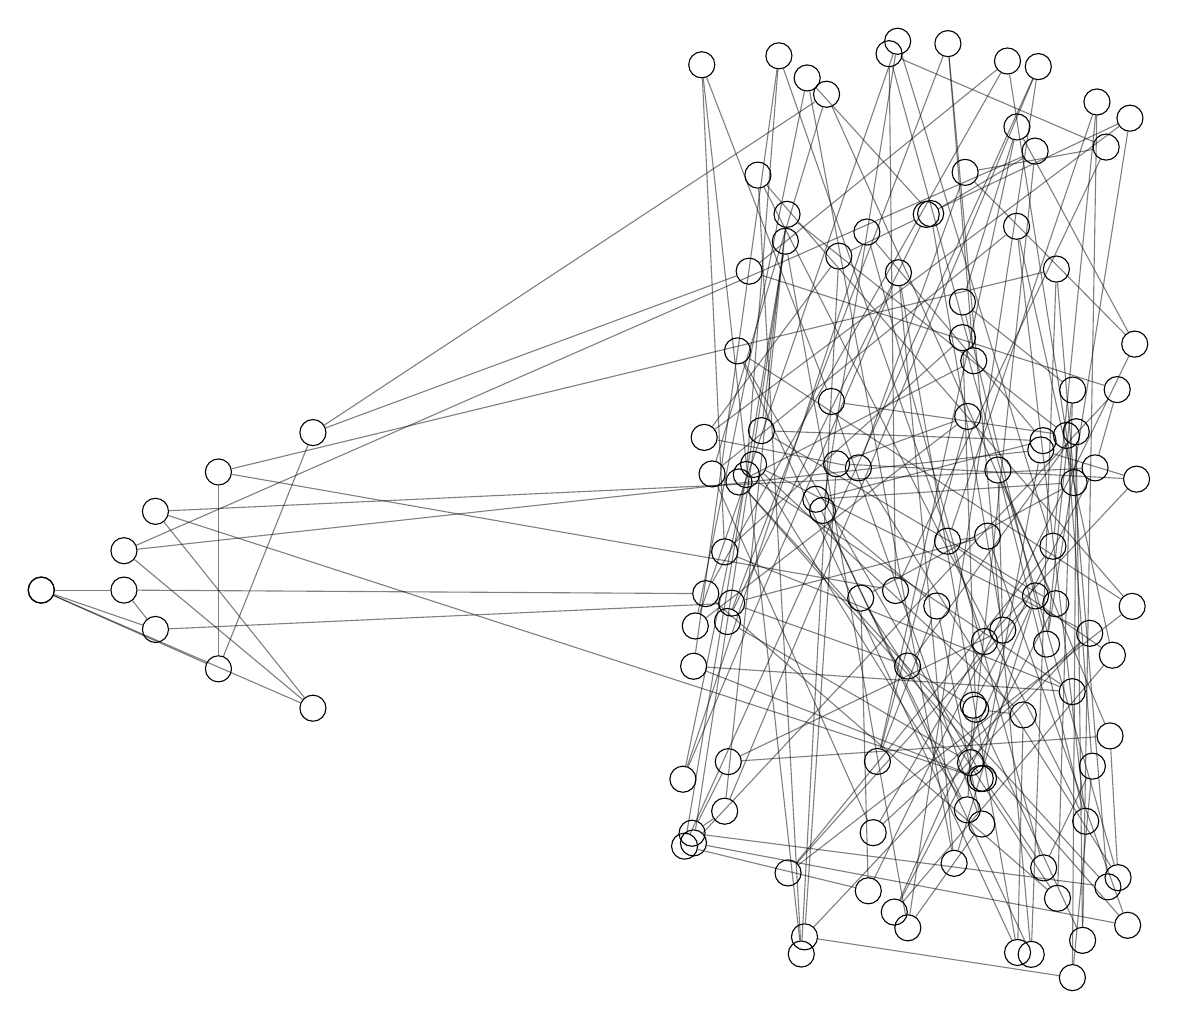
\begin{tikzpicture}[scale=1]
      \draw
        (8.715, 4.601) node[shape=circle,draw=black] (13){}
        (11.801, 2.808) node[shape=circle,draw=black] (88){}
        (9.046, 6.596) node[shape=circle,draw=black] (43){}
        (11.761, 2.209) node[shape=circle,draw=black] (110){}
        (0, 5) node[shape=circle,draw=black] (0){}
        (0, 5) node[shape=circle,draw=black] (51){}
        (12.149, 6.525) node[shape=circle,draw=black] (62){}
        (13.264, 2.064) node[shape=circle,draw=black] (99){}
        (8.99, 9.05) node[shape=circle,draw=black] (101){}
        (3.45, 7.0) node[shape=circle,draw=black] (115){}
        (8.954, 6.468) node[shape=circle,draw=black] (14){}
        (9.368, 11.785) node[shape=circle,draw=black] (22){}
        (10.378, 6.552) node[shape=circle,draw=black] (39){}
        (13.675, 1.348) node[shape=circle,draw=black] (106){}
        (12.017, 5.685) node[shape=circle,draw=black] (48){}
        (11.509, 5.621) node[shape=circle,draw=black] (118){}
        (9.471, 9.772) node[shape=circle,draw=black] (67){}
        (9.146, 7.025) node[shape=circle,draw=black] (98){}
        (11.698, 8.659) node[shape=circle,draw=black] (95){}
        (12.767, 4.314) node[shape=circle,draw=black] (114){}
        (13.383, 6.552) node[shape=circle,draw=black] (68){}
        (1.45, 6.0) node[shape=circle,draw=black] (75){}
        (11.699, 8.206) node[shape=circle,draw=black] (89){}
        (11.867, 3.487) node[shape=circle,draw=black] (107){}
        (10.407, 4.898) node[shape=circle,draw=black] (50){}
        (10.503, 1.181) node[shape=circle,draw=black] (109){}
        (8.419, 6.939) node[shape=circle,draw=black] (73){}
        (10.129, 9.241) node[shape=circle,draw=black] (74){}
        (13.144, 7.011) node[shape=circle,draw=black] (10){}
        (13.225, 0.552) node[shape=circle,draw=black] (100){}
        (11.966, 2.608) node[shape=circle,draw=black] (111){}
        (11.002, 4.035) node[shape=circle,draw=black] (25){}
        (12.892, 9.077) node[shape=circle,draw=black] (34){}
        (2.25, 6.5) node[shape=circle,draw=black] (85){}
        (12.391, 10.882) node[shape=circle,draw=black] (77){}
        (10.619, 2.824) node[shape=circle,draw=black] (83){}
        (12.906, 1.086) node[shape=circle,draw=black] (23){}
        (13.099, 7.54) node[shape=circle,draw=black] (36){}
        (11.766, 7.205) node[shape=circle,draw=black] (69){}
        (10.1, 6.604) node[shape=circle,draw=black] (97){}
        (13.02, 6.964) node[shape=circle,draw=black] (31){}
        (10.035, 7.395) node[shape=circle,draw=black] (58){}
        (1.45, 4.5) node[shape=circle,draw=black] (91){}
        (8.388, 11.671) node[shape=circle,draw=black] (18){}
        (10.767, 11.812) node[shape=circle,draw=black] (52){}
        (11.842, 7.912) node[shape=circle,draw=black] (90){}
        (13.117, 6.365) node[shape=circle,draw=black] (32){}
        (9.837, 6.154) node[shape=circle,draw=black] (87){}
        (9.45, 9.431) node[shape=circle,draw=black] (24){}
        (8.283, 1.789) node[shape=circle,draw=black] (28){}
        (10.833, 0.911) node[shape=circle,draw=black] (7){}
        (12.626, 4.926) node[shape=circle,draw=black] (76){}
        (12.848, 5.557) node[shape=circle,draw=black] (1){}
        (13.407, 11.199) node[shape=circle,draw=black] (35){}
        (11.005, 0.711) node[shape=circle,draw=black] (54){}
        (12.662, 11.648) node[shape=circle,draw=black] (72){}
        (13.546, 1.231) node[shape=circle,draw=black] (33){}
        (8.265, 1.912) node[shape=circle,draw=black] (49){}
        (9.922, 6.011) node[shape=circle,draw=black] (53){}
        (11.373, 4.798) node[shape=circle,draw=black] (82){}
        (12.211, 4.492) node[shape=circle,draw=black] (17){}
        (12.386, 9.62) node[shape=circle,draw=black] (113){}
        (8.17, 1.748) node[shape=circle,draw=black] (20){}
        (9.484, 1.408) node[shape=circle,draw=black] (9){}
        (9.101, 10.27) node[shape=circle,draw=black] (3){}
        (12.271, 11.719) node[shape=circle,draw=black] (80){}
        (12.471, 3.414) node[shape=circle,draw=black] (4){}
        (11.593, 1.53) node[shape=circle,draw=black] (27){}
        (10.886, 9.03) node[shape=circle,draw=black] (93){}
        (1.05, 5.0) node[shape=circle,draw=black] (42){}
        (8.285, 4.033) node[shape=circle,draw=black] (47){}
        (11.925, 2.606) node[shape=circle,draw=black] (105){}
        (12.572, 0.374) node[shape=circle,draw=black] (45){}
        (1.05, 5.5) node[shape=circle,draw=black] (55){}
        (3.45, 3.5) node[shape=circle,draw=black] (63){}
        (12.722, 6.898) node[shape=circle,draw=black] (30){}
        (12.694, 6.78) node[shape=circle,draw=black] (71){}
        (13.91, 6.409) node[shape=circle,draw=black] (81){}
        (10.876, 11.97) node[shape=circle,draw=black] (92){}
        (11.239, 9.771) node[shape=circle,draw=black] (94){}
        (13.826, 10.993) node[shape=circle,draw=black] (119){}
        (13.887, 8.124) node[shape=circle,draw=black] (11){}
        (11.733, 10.305) node[shape=circle,draw=black] (57){}
        (13.797, 0.743) node[shape=circle,draw=black] (15){}
        (12.73, 1.472) node[shape=circle,draw=black] (40){}
        (9.727, 11.504) node[shape=circle,draw=black] (86){}
        (11.836, 3.538) node[shape=circle,draw=black] (64){}
        (8.149, 2.598) node[shape=circle,draw=black] (2){}
        (8.306, 4.544) node[shape=circle,draw=black] (29){}
        (9.973, 11.297) node[shape=circle,draw=black] (26){}
        (12.884, 4.827) node[shape=circle,draw=black] (41){}
        (12.622, 10.575) node[shape=circle,draw=black] (12){}
        (8.842, 8.038) node[shape=circle,draw=black] (6){}
        (13.854, 4.793) node[shape=circle,draw=black] (102){}
        (13.349, 2.764) node[shape=circle,draw=black] (46){}
        (13.095, 0.078) node[shape=circle,draw=black] (65){}
        (11.944, 2.029) node[shape=circle,draw=black] (60){}
        (10.849, 4.995) node[shape=circle,draw=black] (96){}
        (8.768, 4.834) node[shape=circle,draw=black] (79){}
        (13.664, 7.546) node[shape=circle,draw=black] (44){}
        (13.093, 3.71) node[shape=circle,draw=black] (78){}
        (11.514, 11.94) node[shape=circle,draw=black] (38){}
        (11.979, 4.347) node[shape=circle,draw=black] (66){}
        (10.565, 1.919) node[shape=circle,draw=black] (70){}
        (9.652, 0.378) node[shape=circle,draw=black] (103){}
        (8.861, 6.373) node[shape=circle,draw=black] (116){}
        (13.573, 3.148) node[shape=circle,draw=black] (112){}
        (9.693, 0.596) node[shape=circle,draw=black] (59){}
        (13.315, 4.451) node[shape=circle,draw=black] (104){}
        (12.399, 0.398) node[shape=circle,draw=black] (117){}
        (8.725, 2.821) node[shape=circle,draw=black] (84){}
        (10.485, 9.547) node[shape=circle,draw=black] (108){}
        (11.295, 9.782) node[shape=circle,draw=black] (37){}
        (8.679, 2.192) node[shape=circle,draw=black] (21){}
        (8.439, 4.955) node[shape=circle,draw=black] (19){}
        (8.519, 6.475) node[shape=circle,draw=black] (5){}
        (8.679, 5.486) node[shape=circle,draw=black] (61){}
        (13.603, 4.173) node[shape=circle,draw=black] (56){}
        (13.524, 10.626) node[shape=circle,draw=black] (16){}
        (2.25, 4.0) node[shape=circle,draw=black] (8){};
      \begin{scope}[-,draw opacity=0.5]
        \draw (13) to (88);
        \draw (13) to (94);
        \draw (13) to (38);
        \draw (88) to (111);
        \draw (88) to (12);
        \draw (43) to (110);
        \draw (43) to (4);
        \draw (43) to (104);
        \draw (110) to (87);
        \draw (110) to (64);
        \draw (0) to (51);
        \draw (0) to (63);
        \draw (0) to (8);
        \draw (51) to (91);
        \draw (51) to (42);
        \draw (62) to (99);
        \draw (62) to (17);
        \draw (62) to (112);
        \draw (99) to (113);
        \draw (99) to (3);
        \draw (101) to (115);
        \draw (101) to (80);
        \draw (101) to (44);
        \draw (115) to (26);
        \draw (115) to (8);
        \draw (14) to (22);
        \draw (14) to (78);
        \draw (14) to (2);
        \draw (22) to (66);
        \draw (22) to (47);
        \draw (39) to (106);
        \draw (39) to (73);
        \draw (39) to (57);
        \draw (106) to (89);
        \draw (106) to (112);
        \draw (48) to (118);
        \draw (48) to (15);
        \draw (48) to (79);
        \draw (118) to (56);
        \draw (118) to (35);
        \draw (67) to (98);
        \draw (67) to (31);
        \draw (67) to (21);
        \draw (98) to (30);
        \draw (98) to (41);
        \draw (95) to (114);
        \draw (95) to (36);
        \draw (95) to (77);
        \draw (114) to (36);
        \draw (114) to (119);
        \draw (68) to (75);
        \draw (68) to (64);
        \draw (68) to (44);
        \draw (75) to (105);
        \draw (75) to (63);
        \draw (89) to (107);
        \draw (89) to (61);
        \draw (107) to (25);
        \draw (107) to (4);
        \draw (50) to (109);
        \draw (50) to (32);
        \draw (50) to (23);
        \draw (109) to (11);
        \draw (109) to (20);
        \draw (73) to (74);
        \draw (73) to (119);
        \draw (74) to (94);
        \draw (74) to (103);
        \draw (10) to (100);
        \draw (10) to (65);
        \draw (10) to (25);
        \draw (100) to (64);
        \draw (100) to (35);
        \draw (111) to (40);
        \draw (111) to (6);
        \draw (25) to (79);
        \draw (34) to (85);
        \draw (34) to (45);
        \draw (34) to (33);
        \draw (85) to (8);
        \draw (85) to (96);
        \draw (77) to (83);
        \draw (77) to (11);
        \draw (83) to (69);
        \draw (83) to (82);
        \draw (23) to (36);
        \draw (23) to (19);
        \draw (69) to (97);
        \draw (69) to (29);
        \draw (97) to (59);
        \draw (97) to (81);
        \draw (31) to (58);
        \draw (31) to (46);
        \draw (58) to (18);
        \draw (58) to (60);
        \draw (91) to (42);
        \draw (91) to (79);
        \draw (18) to (103);
        \draw (18) to (61);
        \draw (52) to (90);
        \draw (52) to (96);
        \draw (52) to (16);
        \draw (90) to (116);
        \draw (90) to (38);
        \draw (32) to (87);
        \draw (32) to (80);
        \draw (87) to (30);
        \draw (24) to (28);
        \draw (24) to (20);
        \draw (24) to (54);
        \draw (28) to (44);
        \draw (28) to (15);
        \draw (7) to (76);
        \draw (7) to (41);
        \draw (7) to (56);
        \draw (76) to (9);
        \draw (76) to (27);
        \draw (1) to (35);
        \draw (1) to (92);
        \draw (1) to (9);
        \draw (54) to (72);
        \draw (54) to (60);
        \draw (72) to (20);
        \draw (72) to (21);
        \draw (33) to (49);
        \draw (33) to (116);
        \draw (49) to (84);
        \draw (49) to (21);
        \draw (53) to (82);
        \draw (53) to (45);
        \draw (53) to (92);
        \draw (82) to (60);
        \draw (17) to (84);
        \draw (17) to (37);
        \draw (113) to (56);
        \draw (113) to (5);
        \draw (9) to (102);
        \draw (3) to (103);
        \draw (3) to (102);
        \draw (80) to (19);
        \draw (4) to (117);
        \draw (27) to (93);
        \draw (27) to (86);
        \draw (93) to (2);
        \draw (93) to (117);
        \draw (42) to (19);
        \draw (47) to (105);
        \draw (47) to (78);
        \draw (105) to (71);
        \draw (45) to (38);
        \draw (55) to (63);
        \draw (55) to (12);
        \draw (55) to (71);
        \draw (30) to (108);
        \draw (71) to (81);
        \draw (81) to (66);
        \draw (92) to (29);
        \draw (94) to (119);
        \draw (11) to (57);
        \draw (57) to (16);
        \draw (15) to (116);
        \draw (40) to (108);
        \draw (40) to (46);
        \draw (86) to (29);
        \draw (86) to (37);
        \draw (2) to (108);
        \draw (26) to (41);
        \draw (26) to (5);
        \draw (12) to (37);
        \draw (6) to (102);
        \draw (6) to (117);
        \draw (46) to (65);
        \draw (65) to (59);
        \draw (96) to (16);
        \draw (78) to (61);
        \draw (66) to (70);
        \draw (70) to (104);
        \draw (70) to (5);
        \draw (112) to (84);
        \draw (59) to (104);
      \end{scope}
    \end{tikzpicture}
\end{figure}
 
\caption{Expander Graph. Any small set of vertices, like the isolated set on the left, has more edges leaving it than intermediate edges. The exact amount is controlled by the expansion factor.}
\end{figure}
  \begin{theorem*} Theorem, let $C$ be the Tanner Code defined by the small code $C_{0} = [\Delta,\delta\Delta, \rho\Delta ]$ such that $\rho \ge \frac{1}{2}$ and the expander graph $G$ such that $\delta\Delta \ge \lambda$. $C$ is a good  LDPC code.
  \end{theorem*}
  \begin{proof} We have already shown that the graph has a positive rate due to the Tunner construction. So it's left to show also the code has a linear distance. Fix a codeword $x \in C$ and denote By $S$ the support of $x$ over the edges. Namely, a vertex $v\in V$ belongs to $S$ if it connects to nonzero edges regarding the assignment by $x$, Assume towards contradiction that $|x| = o\left( n \right)$. And notice that $|S|$ is at most $2|x|$, Then by The Expander Mixining Lemma we have that: 
  \begin{equation*}
    \begin{split}
      \frac{E\left( S,S \right)}{|S|} & \le \frac{\Delta}{n}|S|  + \lambda \\
      & \le_{ n \rightarrow \infty} o\left( 1 \right) + \lambda
    \end{split}
  \end{equation*}

  Namely, for any such sublinear weight string, $x$, the average of nontrivial edges for the vertex is less than $\lambda$. So there must be at least one vertex $v \in S$ that, on his local view, sets a  string at a weight less than $\lambda$. By the definition of $S$, this string cannot be trivial. Combining the fact that any nontrivial codeword of the $C_{0}$ is at weight at least $\delta\Delta$, we get a contradiction to the assumption that $v$ is satisfied, videlicet, $x$ can't be a codeword \end{proof}

  \subsubsection{Setting $C_{0}$ To Be The Polynomial Code.}
  
  \begin{equation*}
    \begin{split}
     \log \Delta \dim C & \ge \frac{1}{2}n\Delta  - \left( 1- \rho  \right) \Delta n = \frac{1}{2}n\Delta\left( 2\rho - 1 \right)  \\
     \Rightarrow  \dim C & \ge \frac{1}{\log \Delta} \frac{1}{2}n\Delta\left( 2\rho - 1 \right)  
    \end{split}
  \end{equation*}

  \section{Randomized Constructions.}
\begin{claim}
Let $A$ be a random matrix in $M(\mathbb{F}_{2}^{k\times n})$. For any non-zero $x \in \mathbb{F}$, we have that $Ax$ is distributed uniformly.
\end{claim}
\begin{proof}
By the fact that $x \neq 0$, there exists at least one coordinate $i \in [k]$ such that $x_i \neq 0$. Thus, we have
\begin{equation*}
    \begin{split}    
        \left( Ax \right)_{j} &= \sum_{k}{A_{jk}x_{k}} = \sum_{i \neq k}{A_{jk}x_{k}}  + A_{ji}x_{i} \\ 
        & =  \sum_{i \neq k}{A_{jk}x_{k}}  + A_{ji}
      \end{split}
\end{equation*}
Notice that due to the fact that $\mathbb{F}_{2}$ is a field, there is exactly one assignment that satisfies the equation conditioned on all the values $A_{jk}$ where $j \neq k$.    

\begin{equation*}
    \begin{split}
      \prb{\left( Ax \right)_{j} = 1} &=  \sum_{ A_{jk}; k\neq i   }{\prb{\left( Ax \right)_{j} = 1 \mid A_{jk} ; k\neq i }\prb{ A_{jk} ; k\neq i }}  \\
      &= \frac{1}{2} 
    \end{split}
\end{equation*}
Therefore, any coordinate of $Ax$ is distributed uniformly $\Rightarrow$ $Ax$ is distributed uniformly. 
\end{proof}
By the uniformity of $Ax$, we obtain that the expected Hamming weight of $Ax$ is: 
\begin{equation*}
  \begin{split}
    \expp{|Ax| } = \expp{\sum_{i}^{n}{(Ax)_{i}}} = \frac{1}{2} n    
  \end{split}
\end{equation*} 
As the coordinates of $A_{x}$ are independent (each row of $A$ is sampled separately), we can use the Hoff's bound to conclude that: 
\begin{equation*}
  \begin{split}
    \prb{| |Ax| - \expp{|Ax|}| \ge \left(\frac{1}{2} - \delta \right) n } & \le e^{-n \left(\frac{1}{2} - \delta \right)^{2} } 
  \end{split}
\end{equation*}
Now, we will use the union bound to show that any $x \in \mathbb{F}_{2}^{k}$, $Ax$ is of weight at least $\delta$.  
\begin{equation*}
  \begin{split}
    \prb{|Ax| \ge \delta : \forall x \in \mathbb{F}_{2}^{k} } \ge 1 - |\mathbb{F}_{2}^{k}| \cdot e^{-n \left(\frac{1}{2} - \delta \right)^{2} } 
  \end{split}
\end{equation*}
Denote $k = \rho n$ and notice that the above holds when $\rho \ge \left(\frac{1}{2} - \delta \right)^{2} $.  

%
%\subsubsection{Note On Quantum Polynomial Code.} 
%Let's define the code $C$ such that any state in $C$ is a coset of the polynomials at degree at most $d$ shifted by $x \in \mathbb{F}_{p}$. In other words the codeword associated with $x$ is the state $\ket{\underline{c}} = \sum_{ \substack{ f \in \mathbb{F}_{d}[x] \\  f(0) = 0}}{ \ket{ c + f}} $. The inner product between any $d$-degree polynomial with zero free coefficient is:
%\begin{equation*}
%  \begin{split}
%    \braket{ f | x^{j} } = \sum_{i \le d }{ \braket{a_{i} x^{i} | x^{j}}} = \sum_{i \le d}{ a_{i} \expp{ x^{i}x^{j}   }} =  \sum_{i \le d}{ a_{i } \mathbf{1}_{ i + j =_{n} 0 }}
%  \end{split}
%\end{equation*}
%\ctt{Say some words about the classily testability of the polynomial code, and why for quantum it doesn't work. (The dual space of polynomials of low degree is the subspace of all the polynomials with heigh degree.)}
%

